\documentclass{ctexart}

\usepackage{van-de-la-sehen}

\begin{document}

\section{晶体偏振光学} % (fold)
\label{sec:晶体偏振光学}

\subsection{双折射现象} % (fold)
\label{sub:双折射现象}

\subsubsection{基本规律} % (fold)
\label{ssub:基本规律}

一束光入射到介质后变为两束, 则谓发生\emph{双折射}. 折射后的两束光都是线偏振光. 一束光遵守折射定律, 谓寻常光(o光), 另一束不遵守折射定律, 谓非常光(e光).
\par
波矢量$\+vk$的方向始终满足折射定律, 但$\+vS = \+vE\times \+vH$. 由Maxwell方程组可得$\+vD$, $\+vH$, $\+vk$构成右手系, 但$\+vE$和$\+vD$在各向异性介质中不一定同向, 从而$\+vS$和$\+vk$不同向, 故$\+vS$不一定遵守折射定律.
\par
晶体的光轴谓光沿此方向无双折射者. 单轴晶体有方解石晶体, 石英, 冰等, 此时$\+v\epsilon$满足$\epsilon_x = \epsilon_y \neq \epsilon_z$. 双轴晶体有云母, 蓝宝石, 硫磺等, 此时$\epsilon_x \neq \epsilon_y \neq \epsilon_z$. 晶体的单轴与双轴性与晶体的对称性有关. 不发生双折射的晶体, 即$\infty$光轴者, $\epsilon_x = \epsilon_y = \epsilon_z$, 即各向同性.
\par
\begin{figure}[ht]
    \centering
    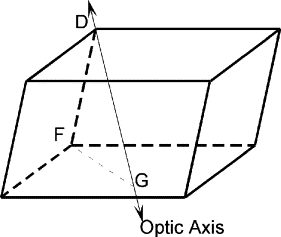
\includegraphics[width=5cm]{src/OpticAxisEg.png}
    \caption{晶体的光轴方向的确定}
    \label{fig:晶体的光轴方向的确定}
\end{figure}
\begin{ex}
    如\cref{fig:晶体的光轴方向的确定}, 方解石的光轴是过三个角都为$\SI{102}{\degree}$的顶点, 三条边的对称轴.
\end{ex}
\begin{pitfall}
    晶体的光轴是一个方向而不是一条线.
\end{pitfall}
\par
主截面为晶体表面的法线与光轴形成的平面.
\begin{pitfall}
    主截面与晶体相关而与光线无关.
\end{pitfall}
\par
晶体中光线与光轴所形成平面谓主平面. o光主平面和e光主平面通常并不重合. o光振动方向垂直于$o$光主平面, e光振动方程平行于e光主平面.
\par
\begin{figure}[ht]
    \centering
    \incfig{8cm}{Principles}
    \caption{蓝线为法线, 红线为光轴, 灰色竖直平面为主截面, 黄蓝平面为主平面.}
\end{figure}
\begin{sample}
    \begin{ex}
        入射光线在主截面内时, 光轴在入射面内. o光, e光主平面与入射面和主截面皆重合. 此时o光偏振严格正交于e光偏振, 若偏振与主平面之间成$\theta$角度, 则
        \[ E_o = E\sin\theta,\quad E_e = E\cos\theta,\quad I_o = I\sin^2\theta,\quad I_e = I\cos^2\theta. \]
    \end{ex}
\end{sample}

% subsubsection 基本规律 (end)

\subsubsection{单轴晶体中的波面} % (fold)
\label{ssub:单轴晶体中的波面}

Huygens作图法要求
\begin{cenum}
    \item 波面以速度$v$推进;
    \item 晶体中将有o, e两个次波波面;
    \item o光的波面是球面, e光的波面是椭球面;
    \item 用点(垂直纸面)和线段(面内)代表偏振.
\end{cenum}
\begin{figure}[ht]
    \centering
    \begin{subfigure}{4.1cm}
        \centering
        \incfig{4.1cm}{WaveFrontO}
        \caption{o光波前} 
    \end{subfigure}
    \begin{subfigure}{6cm}
        \centering
        \incfig{6cm}{WaveFrontE}
        \caption{e光波前} 
    \end{subfigure}
    \caption{负晶体中o光和e光在晶体中的波前}
\end{figure}
\begin{figure}[ht]
    \centering
    \begin{subfigure}{4.1cm}
        \centering
        \incfig{4.1cm}{WaveFrontO}
        \caption{o光波前} 
    \end{subfigure}
    \begin{subfigure}{6cm}
        \centering
        \incfig{2.82cm}{PosWaveFrontE}
        \caption{e光波前} 
    \end{subfigure}
    \caption{正晶体中o光和e光在晶体中的波前}
\end{figure}
因此, e光只有在两个正交方向上才有波面和传播方向垂直. e光的速度在各个方向都不相同. 若e光沿与光轴垂直方向传播的速度为$v_e$, 则其主折射率为$n_e = c/v_e$.
\begin{cenum}
    \item 若$v_e > v_o$, $n_e < n_o$, 则谓之负晶体; 例如冰洲石.
    \item 若$v_e < v_o$, $n_e > n_o$, 则谓之正晶体; 例如石英.
\end{cenum}
在正交于光轴的各个方向上, e光传播的速度相同, 故波前的投影为圆.

\begin{figure}[ht]
    \centering
    \begin{subfigure}{5cm}
        \centering
        \incfig{4.7cm}{Huygens1}
        \caption{}
        \label{fig:HuygensStep1}
    \end{subfigure}
    \begin{subfigure}{5cm}
        \centering
        \incfig{4.7cm}{Huygens2}
        \caption{}
        \label{fig:HuygensStep2}
    \end{subfigure}
    \begin{subfigure}{5cm}
        \centering
        \incfig{4.7cm}{Huygens3}
        \caption{}
        \label{fig:HuygensStep3}
    \end{subfigure}
    \begin{subfigure}{5cm}
        \centering
        \incfig{4.7cm}{Huygens4}
        \caption{}
        \label{fig:HuygensStep4}
    \end{subfigure}
    \caption{Huygens作图法}
\end{figure}

\paragraph{Huygens作图法} % (fold)
\label{par:huygens作图法}

若光轴在入射面内,
\begin{cenum}
    \item 如\cref{fig:HuygensStep1}, 作出入射光的波面, 当$2$到达界面$B$点时, $A$点的光已经在介质中传播$t = BB'/c$.
    \item 如\cref{fig:HuygensStep2}, 以$A$为中心, $v_ot$为半径作球面, 该球面过$B'$的平面的切点为$A'_o$, 则$AA'_o$即为o光的方向.
    \item 如\cref{fig:HuygensStep3}, 以上一步的圆中沿光轴方向的直径作为一轴, 垂直方向上长度为$v_et$的线段作为另一轴, 作一椭圆.
    \item 如\cref{fig:HuygensStep4}, 过$B$作上一步中的椭球面的切点$A'_e$, 则$AA'_e$为e光的方向.
\end{cenum}

% paragraph huygens作图法 (end)

\begin{figure}[ht]
    \centering
    \incfig{6cm}{NormalIncidentAlongOpticalAxis}
    \caption{}
    \label{fig:光轴垂直于界面的正入射}
\end{figure}
\begin{sample}
    \begin{ex}
        如\cref{fig:光轴垂直于界面的正入射}, 光轴垂直于界面的正入射情形下, 不发生双折射.
    \end{ex}
\end{sample}
\begin{figure}[ht]
    \centering
    \incfig{6cm}{NormalIncidentOrthoOpticalAxis}
    \caption{}
    \label{fig:光轴平行于界面的正入射}
\end{figure}
\begin{sample}
    \begin{ex}
        如\cref{fig:光轴平行于界面的正入射}, o光和e光方向一致但会产生相位差.
    \end{ex}
\end{sample}
\begin{figure}[ht]
    \centering
    \incfig{6cm}{ObliqueIncidentOrthoOpticalAxis}
    \caption{}
    \label{fig:光轴垂直于入射面的斜入射}
\end{figure}
\begin{sample}
    \begin{ex}
        如\cref{fig:光轴垂直于入射面的斜入射}, 光轴垂直于入射面, 斜入射, 则
        \[ n\sin\theta = n_o\sin\theta_o = n_e\sin\theta_e. \]
    \end{ex}
\end{sample}
\begin{figure}[ht]
    \centering
    \begin{subfigure}{5cm}
        \centering
        \incfig{5cm}{NegCrystalNormal}
        \caption{负晶体正入射折射}
    \end{subfigure}
    \begin{subfigure}{5cm}
        \centering
        \incfig{5cm}{PosCrystalNormal}
        \caption{正晶体正入射折射}
    \end{subfigure}
    \caption{}
    \label{fig:正负晶体正入射折射}
\end{figure}
\begin{sample}
    \begin{ex}
        根据折射情况判断晶体正负.
    \end{ex}
    \begin{solution}
        如\cref{fig:正负晶体正入射折射}, 将两种情况画出的折射光线分别作图, 与条件对比, 符合者为正确情形.
    \end{solution}
\end{sample}

% subsubsection 单轴晶体中的波面 (end)

% subsection 双折射现象 (end)

\subsection{晶体光学器件} % (fold)
\label{sub:晶体光学器件}

\subsubsection{晶体偏振器} % (fold)
\label{ssub:晶体偏振器}

\begin{figure}[ht]
    \centering
    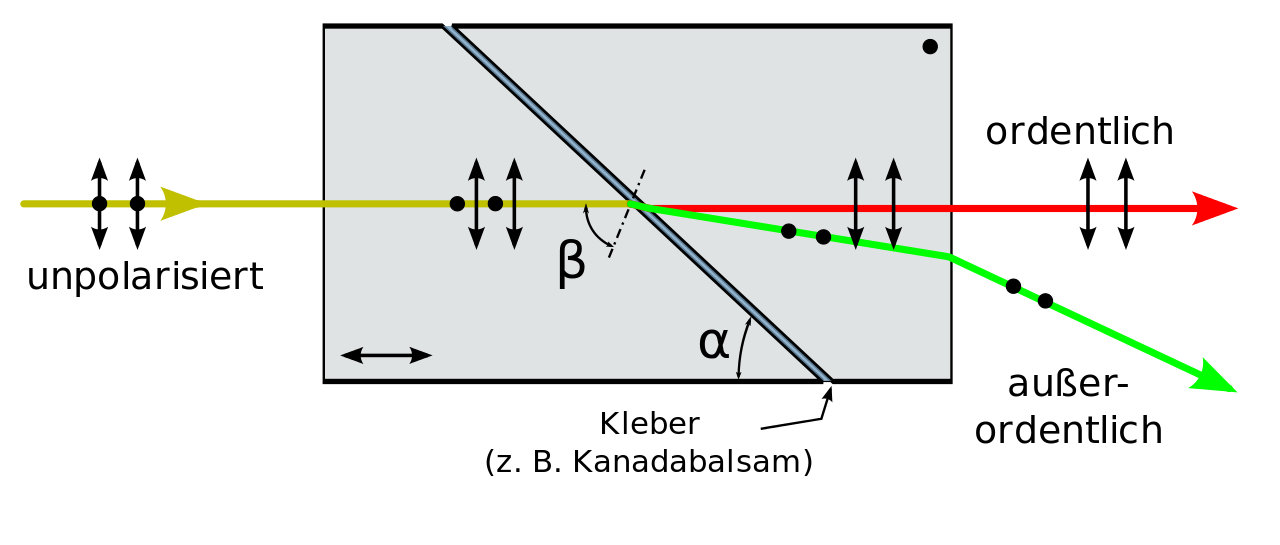
\includegraphics[width=9cm]{src/Rochon.png}
    \caption{Rochon棱镜}
\end{figure}

\paragraph{Rochon棱镜} % (fold)
\label{par:rochon棱镜}

由冰洲石作成直角三棱镜粘合而成.
\begin{cenum}
    \item 在$1$区, 入射光沿着光轴;
    \item 在$2$区, 入射线垂直于光轴, 在主截面内;
    \begin{cenum}
        \item o光的$v_o$不变;
        \item v光的$v_e\neq v_0$, 发生偏折.
    \end{cenum}
\end{cenum}
遮挡其中一束, 得到线偏光.

% paragraph rochon棱镜 (end)

\begin{figure}[ht]
    \centering
    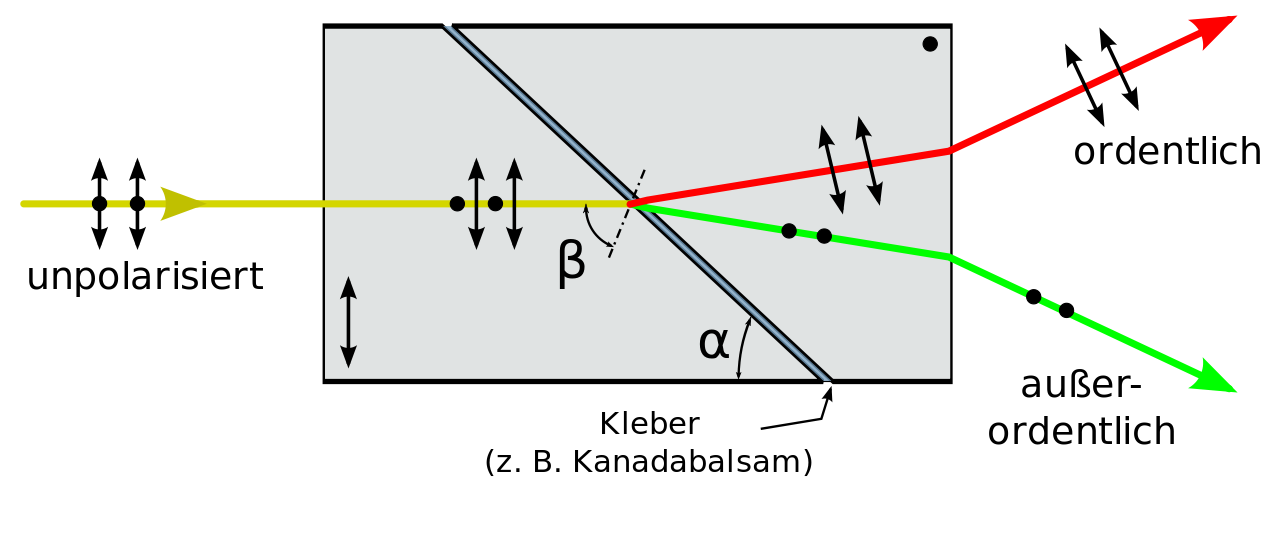
\includegraphics[width=9cm]{src/Wollaston.png}
    \caption{Wollaston棱镜}
\end{figure}

\paragraph{Wollaston棱镜} % (fold)
\label{par:wollaston棱镜}

构造与Rochon棱镜类似.
\begin{cenum}
    \item 在$1$区, 入射光垂直于光轴, $v_0\neq v_e$;
    \item 在$2$区, o和e互换, 两者均发生折射.
\end{cenum}

% paragraph wollaston棱镜 (end)

\begin{figure}[ht]
    \centering
    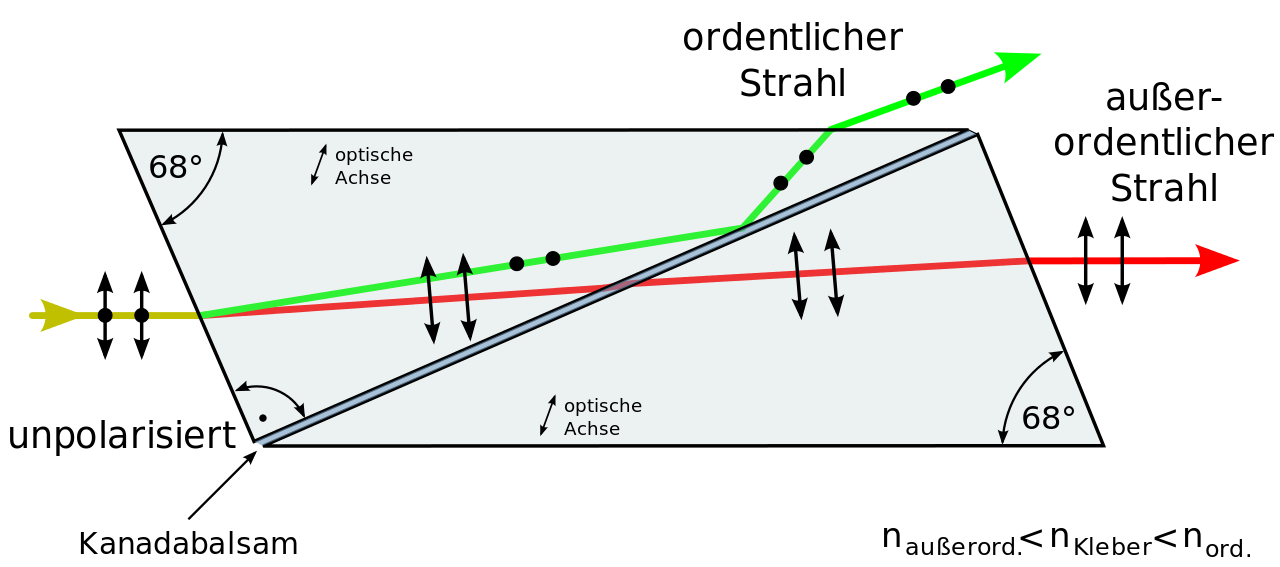
\includegraphics[width=9cm]{src/Nicol.png}
    \caption{Nicol棱镜}
\end{figure}

\paragraph{Nicol棱镜} % (fold)
\label{par:nicol棱镜}

将冰洲石斜切开, 使得切开面垂直于主截面, 之后用加拿大树胶粘合, 在顶部吸收o光, 即可得到出射e光.
\[ n_e < n_o,\quad i_c = \arcsin \frac{n_{\text{胶}}}{n}. \]

\begin{remark}
    Nicol棱镜并非正入射, 几何结构复杂.
\end{remark}

% paragraph nicol棱镜 (end)

\begin{figure}[ht]
    \centering
    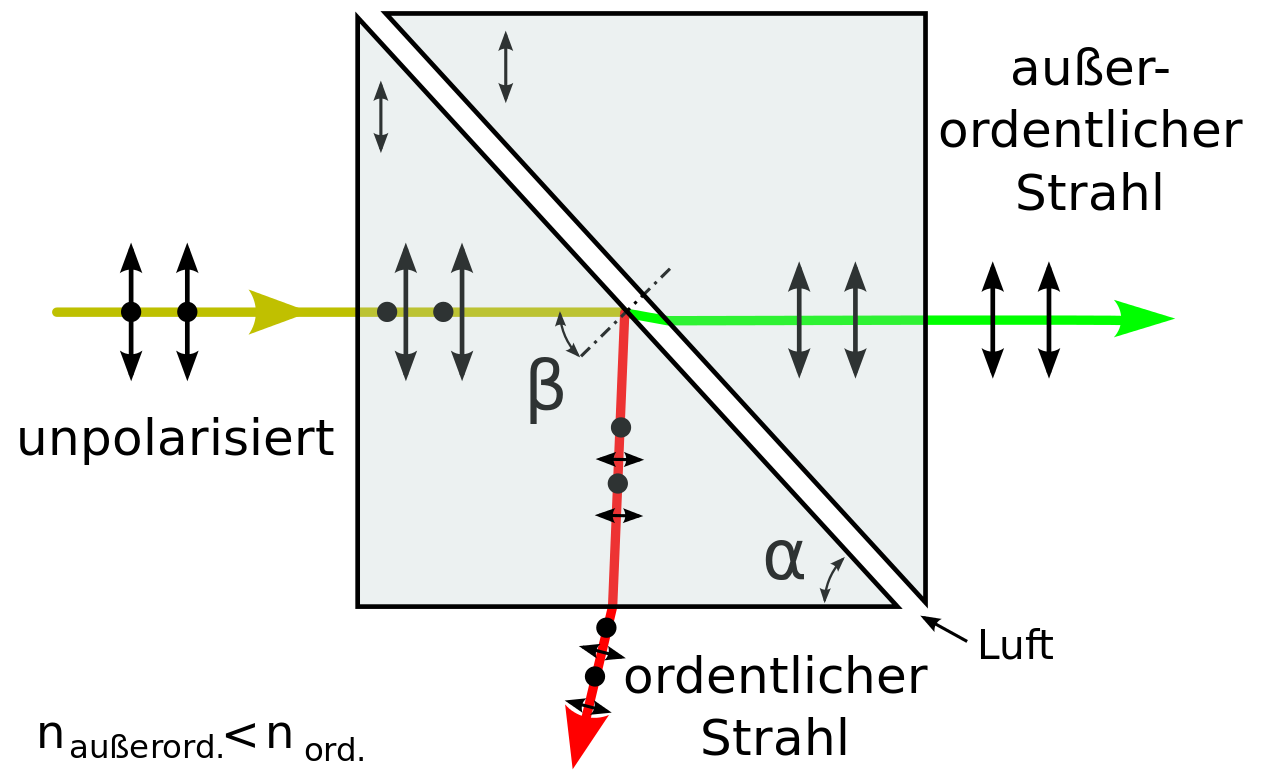
\includegraphics[width=9cm]{src/GlanTaylor.png}
    \caption{Glan-Taylor棱镜}
\end{figure}

\paragraph{Glan-Taylor棱镜} % (fold)
\label{par:glan_taylor棱镜}

采用冰洲石晶体, 选择合适切角, 中间采用空气间隙. o光和e光的折射率不同, 选择合适切角可以让入射光束中的o光成分在内部的玻璃-空气界面发生全反射. 剩下只有e光成分可以通过偏振器.
\par
在$1$区垂直于光轴方向传播, 设
\begin{align*}
    n_o &= 1.66,\quad n_e = 1.49, \\
    i_{co} &= \arcsin \rec{n_0} = \SI{37}{\degree}, \\
    i_{ce} &= \arcsin \rec{n_e} = \SI{42}{\degree}.
\end{align*}

% paragraph glan_taylor棱镜 (end)

% subsubsection 晶体偏振器 (end)

\subsubsection{波片} % (fold)
\label{ssub:波片}

\begin{figure}[ht]
    \centering
    \incfig{6cm}{WavePlate}
    \caption{波片}
    \label{fig:波片}
\end{figure}
波片的构造如\cref{fig:波片}, 光轴与界面表面平行, 故
\[ \Delta = \varphi_o - \varphi_e = \frac{2\pi}{\lambda}\pare{n_o - n_e}d. \]
$\lambda/4$波片要求
\[ \pare{n_o - n_e}d = \frac{\lambda}{4} + n\lambda, \]
$\lambda/2$波片要求
\[ \pare{n_o - n_e}d = \frac{\lambda}{2} + n\lambda. \]
零阶波片要求$n=0$.

\begin{figure}[ht]
    \centering
    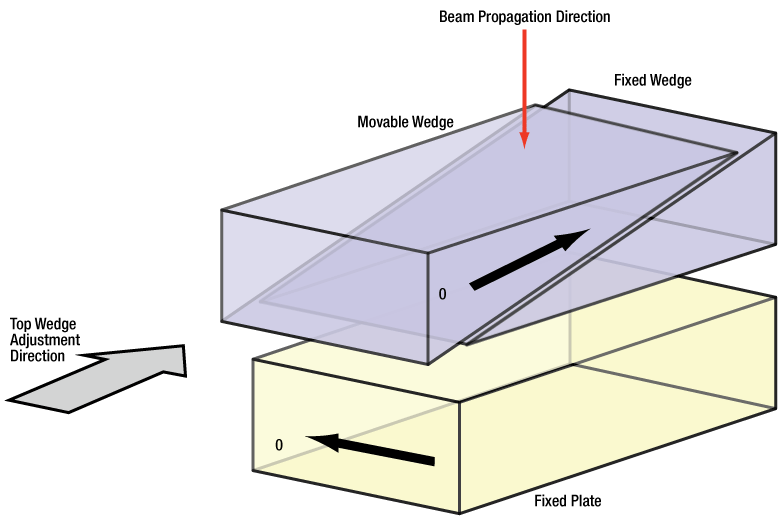
\includegraphics[width=11cm]{src/BabinetSoleil.png}
    \caption{Babinet-Soleil补偿器}
    \label{fig:babinet-soleil补偿器}
\end{figure}

\paragraph{Babinet-Soleil补偿器} % (fold)
\label{par:babinet_soleil补偿器}

补偿器之构造如\cref{fig:babinet-soleil补偿器}, 粘合楔形波片,
\begin{align*}
    \Delta \varphi &= \frac{2\pi}{\lambda} \brac{\pare{n_o - n_e}d_1 + \pare{n_e - n_o}d_2} \\
    &= \frac{2\pi}{\lambda}\pare{n_o - n_e}\pare{d_1-d_2}.
\end{align*}

% paragraph babinet-soleil补偿器 (end)

\paragraph{作业} % (fold)
\label{par:作业}

p.181 1,2,3 (p.390), p.187 1,2,3 (p.394)

% paragraph 作业 (end)

% subsubsection 波片 (end)

% subsection 晶体光学器件 (end)

\subsection{检偏} % (fold)
\label{sub:检偏}

\subsubsection{垂直振动的合成} % (fold)
\label{ssub:垂直振动的合成}

若$E_x$和$E_y$有相位差,
\[ \begin{cases}
    E_x = A_x \cos \omega t \sim A_x e^{i\omega t}, \\
    E_y = A_y \cos\pare{\omega t + \delta} \sim A_y e^{i\pare{\omega t + \delta}},
\end{cases} \]
\begin{figure}[ht]
    \centering
    \incfig{8cm}{CounterPolar}
    \caption{左旋光合成}
    \label{fig:左旋光合成}
\end{figure}
\begin{figure}[htb]
    \centering
    \incfig{6cm}{GeneralElliptic}
    \caption{一般椭圆偏振光的合成}
    \label{fig:一般椭圆偏振光的合成}
\end{figure}
\begin{cenum}
    \item $\delta = 0, \pi$时有线偏光特例, $\displaystyle \tan\theta = \pm \frac{A_y}{A_x}$.
    \item 当$\delta = \pi/2$时有椭圆偏振特例,
    \[ \pare{\frac{E_x}{A_x}}^2 + \pare{\frac{E_y}{A_y}}^2 = 1. \]
    当$\delta = \pi/2$为右旋, $\delta = -\pi/2$为左旋(如\cref{fig:左旋光合成}), $A_x=A_y$时为圆偏.
    \item 对于一般的椭圆偏振, 如\cref{fig:一般椭圆偏振光的合成}, 椭圆并非正置, 在$E_x = \pm A_x$和$E_y = \pm A_y$处与平行于坐标轴的直线相切. 轨迹方程
    \[ \frac{E_x^2}{A_x^2} + \frac{E_y^2}{A_y^2} - \frac{2E_xE_y}{A_xA_y} \cos\delta = \sin^2\delta. \]
    主轴方向
    \[ \tan 2\alpha = \frac{2A_xA_y}{A_x^2 - A_y^2}\cos\delta. \]
    当$-\pi < \delta < 0$时合成光为左旋, $0<\delta<\pi$时为右旋.
\end{cenum}

% subsubsection 垂直振动的合成 (end)

\subsubsection{圆偏振和椭圆偏振的获得} % (fold)
\label{ssub:圆偏振和椭圆偏振的获得}

将线偏光通过波片, 则一侧偏振发生$\delta$的相位延迟,
\[ E_x = A_x e^{i\omega t},\quad E_y = A_y e^{i\pare{\omega t + \delta}},\quad \delta = \frac{2\pi}{\lambda}\pare{n_o - n_e}d. \]
在一般情形下获得的光是椭圆偏振光. 如果采用$1/4$波片且$A_o = A_e$, 则产生圆偏光.

% subsubsection 圆偏振和椭圆偏振的获得 (end)

\subsubsection{圆偏振和椭圆偏振经过检偏器后的强度变化} % (fold)
\label{ssub:圆偏振和椭圆偏振经过检偏器后的强度变化}

\begin{figure}[htb]
    \begin{subfigure}[b]{6cm}
    \centering
    \incfig{6cm}{GeneralEllipticPassingThroughPolarizer}
    \caption{}
    \label{fig:椭圆偏过检偏器}
    \end{subfigure}
    \begin{subfigure}[b]{6cm}
    \centering
    \incfig{6cm}{GeneralEllipticPassingThroughWavePlate}
    \caption{}
    \label{fig:椭圆偏振过波片}
    \end{subfigure}
    \caption{}
\end{figure}
如\cref{fig:椭圆偏过检偏器}, 假设检偏器与$x$成$\alpha$角, $\displaystyle \begin{cases}
            E_x = A_x e^{i\omega t}, \\
            E_y = A_y e^{i\pare{\omega t + \delta}},
        \end{cases}$ 则
\begin{align*}
    E &= A_x \cos\alpha e^{i\omega t} + A_y \sin \alpha e^{i\pare{\omega t + \delta}} = \pare{A_x\ cos\alpha + A_y \sin \alpha e^{i\delta}}e^{i\omega t}, \\
    I &= E^*E = A_x^2 \cos^2\alpha + A_y^2 \sin^2\alpha + A_xA_y \sin 2\alpha \cos\delta.
\end{align*}

% subsubsection 圆偏振和椭圆偏振经过检偏器后的强度变化 (end)

\subsubsection{出射偏振态的改变} % (fold)
\label{ssub:出射偏振态的改变}

为求出出射波片的偏振态,
\begin{cenum}
    \item 将入射光按波片的o光和e光分解, 求出o光和e光的振幅和相位差.
    \item 计算由波片导致的o光和e光的相位差.
    \item 合成出射的o光和e光.
\end{cenum}
\begin{sample}
    \begin{ex}
        如\cref{fig:椭圆偏振过波片}, 假设入射光为右旋偏振, 求$1/4$波片的光轴与椭圆长轴的夹角为$0$, $\SI{90}{\degree}$和$\SI{45}{\degree}$度时的偏振态. 设o光延迟$\pi/2$.
    \end{ex}
    \begin{solution}
        右旋椭圆偏振光
        \[ \delta = \pi/2, \quad A_x \neq A_y, \quad \begin{cases}
            E_x = A_x e^{i\omega t}, \\
            E_y = A_y e^{i\pare{\omega t + \delta}}.
        \end{cases} \]
        入射时
        \[ \begin{cases}
            E_e = \pare{A_x \cos\alpha + A_y\sin\alpha e^{i\delta}}e^{i\omega t}, \\
            E_o = \pare{-A_x\sin\alpha + A_y\cos\alpha e^{i\delta}}e^{i\omega t}.
        \end{cases} \]
        经过$1/4$波片后, 引入$\Delta = \pi/2$的相位差, 出射时
        \[ \begin{cases}
            E_e = \pare{A_x \cos\alpha + A_y\sin\alpha e^{i\delta}}e^{i\omega t}, \\
            E_o = \pare{-A_x\sin\alpha + A_y\cos\alpha e^{i\delta}}e^{i\Delta}e^{i\omega t}.
        \end{cases} \]
        $\alpha = \SI{0}{\degree}$或$\alpha = \SI{90}{\degree}$相当于椭圆长短轴对其了$e$轴和$o$轴, 出射为线偏光.
    \end{solution}
    \begin{remark}
        光轴方向即e光的偏振方向.
    \end{remark}
\end{sample}

% subsubsection 出射偏振态的改变 (end)

\subsubsection{各种偏振的检验} % (fold)
\label{ssub:各种偏振的检验}

注意如下事实:
\begin{cenum}
    \item 线偏光经过$1/4$波片产生椭圆偏振光.
    \item 圆偏光经过$1/4$波片得到线偏光.
    \item $\delta = \pi/2$的正椭圆偏振光, 长轴对齐$1/4$波片的光轴得到线偏光.
    \item 对于一般的$\delta$, 仍然得到椭圆偏振.
\end{cenum}
因此, 检偏之一般步骤如
\begin{cenum}
    \item 使用线检偏器, 可以鉴定线偏振光. 转动检偏器, 线偏光会发生消光, 而圆偏振和自然偏振不发生光强改变, 椭圆偏振和部分偏振会发生光强改变但是不会消光.
    \item 直接让入射光通过通过$1/4$波片, 自然光和部分偏振光不变, 圆偏振变为线偏振光, 椭圆偏振光仍然得到椭圆偏振光, 当光轴与椭圆长短轴符合则得到线偏光.
    \item 再通过偏振片, 就可以区分自然光/圆偏光以及部分偏振光/椭圆偏振光.
\end{cenum}

\paragraph{半波片的作用} % (fold)
\label{par:半波片的作用}

椭圆偏振光经过半波片, 将产生$\pm \pi$的额外相位差, 导致反相从而旋转方向相反. 实际上, 这导致光的偏振沿着$o$轴反射. 若使用圆偏光经过, 则产生则直接导致旋转方向改变.
\par
若采用线偏光入射, 则出射光偏振方向沿着$o$轴反射.

% paragraph 半波片的作用 (end)

\begin{longtable}{|c|c|c|}
    \hline
    光 & QWP& HWP \\
    \hline
    自然光 & 自然光 & 自然光 \\
    \hline
    圆偏光 & 线偏光 & 反向旋转 \\
    \hline
    线偏光 & 一般为椭偏 & $2\theta$转动 \\
    \hline
    椭偏光 & 一般为椭偏 & 反向旋转 \\
    \hline
    部分偏振光 & 部分偏振光 & 部分偏振光 \\
    \hline
    \caption{不同类型的偏振光经过QWP和HWP的结果}
    \label{fig:不同类型的偏振光经过QWP和HWP的结果}
\end{longtable}
从\cref{fig:不同类型的偏振光经过QWP和HWP的结果}出发可以得到鉴别五种偏振光的方式.
\begin{remark}
    教材中对相位符号的约定为
    \[ E_o\pare{P} \cos \brac{\omega t - \varphi\pare{P}} \mapsto A\pare{P} e^{i\varphi\pare{P}}e^{-i\omega t}. \]
    经过波片后, $\varphi_o = 2\pi n_od/\lambda$, $\varphi_e = 2\pi n_e d/\lambda$. 则
    \begin{align*}
        & A_0 e^{i\varphi_o} + Ae^{i\varphi_e} \\
        &= e^{i\varphi_o} \pare{A_o + A_e e^{i\pare{\varphi_e - \varphi_o}}} \\
        &= e^{i\varphi_e} \pare{A_e + A_o e^{i\pare{\varphi_o - \varphi_e}}}.
    \end{align*}
\end{remark}

% subsubsection 各种偏振的检验 (end)

\subsubsection{Jones表述} % (fold)
\label{ssub:jones表述}

参考\href{https://en.wikipedia.org/wiki/Jones_calculus}{Jones calculus}. 若$\ket{H}$用$\begin{pmatrix}
    0 & 1
\end{pmatrix}^T$表示, $\ket{V}$用$\begin{pmatrix}
    1 & 0
\end{pmatrix}^T$表示. 则入射光的偏振可以用
\[ \alpha \ket{H} + \beta\ket{V},\quad \abs{\alpha}^2 + \abs{\beta}^2 = 1 \]
表示. 任意偏振可以表示为$\begin{pmatrix}
    \cos\theta & \sin\theta e^{i\varphi}
\end{pmatrix}^T$. 故半波片的操作相当于
\[ \ket{H} \mapsto \cos 2\theta \ket{H} + \sin 2\theta\ket{V},\quad \ket{V} \mapsto \sin 2\theta \ket{H} - \cos 2\theta \ket{V}. \]
欲求出$1/4$波片的操作矩阵, 先将光在o和e的轴向上分解, 再换回以$\ket{H}$和$\ket{V}$为基矢.
\begin{align*}
    \ket{H} \mapsto \ket{\psi_H} &= \cos \theta \ket{e} + \sin\theta \ket{o} e^{-i\pi/2} \\
    &= \cos\theta \pare{\cos\theta \ket{H} + \sin\theta\ket{V}} - i\sin\theta\pare{-\sin\theta \ket{H} + \cos\theta\ket{V}} \\
    &= \pare{\cos^2\theta + i\sin^2\theta}\ket{H} + \pare{\pare{1-i}\sin\theta\cos\theta}\ket{V}.
\end{align*}
故操作矩阵为
\[ \begin{pmatrix}
  \cos^2\theta + i\sin^2\theta & (1 - i)\sin\theta \cos\theta \\
  (1 - i)\sin\theta \cos\theta & \sin^2\theta + i\cos^2\theta
\end{pmatrix}. \]
多个波片连续放置, 则将多个矩阵连乘即可.
\begin{sample}
    \begin{ex}
        若干入射光经过$\SI{0}{\degree}$的$1/4$波片的效果如
        \begin{align*}
            \rec{\sqrt{2}} \begin{pmatrix}
                1 \\ 1
            \end{pmatrix} &\mapsto \rec{\sqrt{2}}\begin{pmatrix}
                1 \\ i
            \end{pmatrix}. \\
            \rec{\sqrt{2}} \begin{pmatrix}
                1 \\ -1
            \end{pmatrix} &\mapsto \rec{\sqrt{2}}\begin{pmatrix}
                1 \\ -i
            \end{pmatrix}. \\
            \rec{\sqrt{2}} \begin{pmatrix}
                1 \\ i
            \end{pmatrix} &\mapsto \rec{\sqrt{2}}\begin{pmatrix}
                1 \\ -1
            \end{pmatrix}.
        \end{align*}
    \end{ex}
\end{sample}
\begin{sample}
    \begin{ex}
        对于$\SI{45}{\degree}$的半波片, 有操作矩阵$\displaystyle \begin{pmatrix}
            0 & 1 \\ 1 & 0
        \end{pmatrix}$, 从而
        \begin{align*}
            \begin{pmatrix}
                1 & 0
            \end{pmatrix} & \mapsto \begin{pmatrix}
                0 & 1
            \end{pmatrix}, \\
            \begin{pmatrix}
                1 & 1
            \end{pmatrix} & \mapsto \begin{pmatrix}
                1 & 1
            \end{pmatrix}.
        \end{align*}
        $\SI{0}{\degree}$的半波片有操作矩阵$\displaystyle \begin{pmatrix}
            1 & 0 \\ 0 & -1
        \end{pmatrix}$, 从而
        \[ \begin{pmatrix}
                1 & 1
            \end{pmatrix}  \mapsto \begin{pmatrix}
                1 & -1
            \end{pmatrix}. \]
    \end{ex}
\end{sample}

\paragraph{作业} % (fold)
\label{par:作业}

p.201 1, 2, 3 (p.404)

% paragraph 作业 (end)

% subsubsection jones表述 (end)

% subsection 检偏 (end)

\subsection{偏振光干涉及其应用} % (fold)
\label{sub:偏振光干涉及其应用}

\subsubsection{偏振器间的波晶片} % (fold)
\label{ssub:偏振器间的波晶片}

\begin{figure}[htb]
    \centering
    \incfig{10cm}{WavePlateBetweenPolarizers}
    \caption{偏振片之间放入波片}
    \label{fig:偏振片之间放入波片}
\end{figure}
如\cref{fig:偏振片之间放入波片}, 在两个偏振片I和II之间插入一块厚度为$d$的波晶片, 则经过波晶片时, 若设e轴与$P_1$轴的夹角为$\alpha$, 如\cref{fig:偏振片之间放入波片坐标系},
\[ A_e = A_1\cos\alpha,\quad A_o = -A_1\sin\alpha. \]
\begin{figure}[t]
    \begin{subfigure}{5cm}
    \centering
    \incfig{5cm}{WavePlateBetweenPolarizersCoor}
    \caption{}
    \label{fig:偏振片之间放入波片坐标系}
    \end{subfigure}
    \hspace{1.5cm}
    \begin{subfigure}{5cm}
    \centering
    \incfig{5cm}{WavePlateBetweenPolarizersCoor2}
    \caption{}
    \label{fig:偏振片之间放入波片坐标系2}
    \end{subfigure}
    \caption{}
\end{figure}
若设$P_2$与e轴的夹角为$\beta$, 如\cref{fig:偏振片之间放入波片坐标系2}, 则
\[ A_{e2} = A_e\cos\beta = A_1\cos\alpha\cos\beta,\quad A_{o2} = A_o\sin\beta = -A_1\sin\alpha\sin\beta. \]
合成后
\[ \+vE_2 = \+vE_{e2} + \+vE_{o2} = A_{e2} + A_{o2}e^{i\delta} = A_1\cos\alpha\cos\beta - A_1\sin\alpha\sin\beta e^{i\delta}. \]
$I_2 = \+vE_2\+vE_2^*$和$\alpha,\beta,\delta$有关,
\begin{align*}
    I_2 &= A_1^2\brac{\cos^2\alpha\cos^2\beta + \sin^2\alpha\sin^2\beta - 2\cos\alpha\cos\beta\sin\alpha\sin\beta\cos\Delta}, \\
    \Delta &= \frac{2\pi}{\lambda}\pare{n_o - n_e} d.
\end{align*}
\begin{figure}[ht]
    \centering
    \begin{subfigure}{5cm}
        \centering
        \incfig{5cm}{SpecialCaseOrtho45}
        \caption{}
        \label{fig:双偏振片例1}
    \end{subfigure}
    \begin{subfigure}{5cm}
        \centering
        \incfig{5cm}{SpecialCasePara45}
        \caption{}
        \label{fig:双偏振片例2}
    \end{subfigure}
\end{figure}
\begin{sample}
    \begin{ex}
        如\cref{fig:双偏振片例1}, $\alpha = \beta = \SI{45}{\degree}$, $P_1\perp P_2$, 则
        \[ I_2 = \frac{A_1^2}{2}\pare{1-\cos\Delta}. \]
    \end{ex}
\end{sample}
\begin{sample}
    \begin{ex}
        如\cref{fig:双偏振片例2}, $\alpha = \beta = \SI{45}{\degree}$, $P_1 \parallelsum P_2$, 则
        \[ I_2 = \frac{A_1^2}{2}\pare{1+\cos\Delta}. \]
    \end{ex}
\end{sample}

% subsubsection 偏振器间的波晶片 (end)

\subsubsection{显色偏振} % (fold)
\label{ssub:显色偏振}

自然光入射到厚度均匀的波片,
\begin{cenum}
    \item $\displaystyle \Delta_1 = \frac{2\pi}{\lambda_1}\pare{n_o - n_e}d = 2k\pi$,
    \begin{cenum}
        \item $P_1\perp P_2$, $I_2 = 0$, 显示$\lambda_1$的互补色;
        \item $P_1\parallelsum P_2$, $I_2 = A_1^2$, 显示$\lambda_1$的颜色.
    \end{cenum}
    \item $\displaystyle \Delta_2 = \frac{2\pi}{\lambda_2}\pare{n_o -  n_e}d = \pare{2k+1}\pi$,
    \begin{cenum}
        \item $P_1\perp P_2$, $I_2 = A_1^2$, 显示$\lambda_2$的颜色;
        \item $P_1\parallelsum P_2$, $I_2 = 0$, 显示$\lambda_2$的互补色.
    \end{cenum}
\end{cenum} 

% subsubsection 显色偏振 (end)

\subsubsection{偏振光干涉} % (fold)
\label{ssub:偏振光干涉}

单色光入射到楔形波片,
\begin{cenum}
    \item $\displaystyle \Delta_1 = \frac{2\pi}{\lambda}\pare{n_o - n_e}d_1 = 2k\pi$,
    \begin{cenum}
        \item $P_1\perp P_2$, 暗条纹;
        \item $P_1\parallelsum P_2$, 条纹明暗互换.
    \end{cenum}
    \item $\displaystyle \Delta_2 = \frac{2\pi}{\lambda}\pare{n_o - n_e}d_2 = \pare{2k+1}\pi$,
    \begin{cenum}
        \item $P_1\perp P_2$, 亮条纹;
        \item $P_1\parallelsum P_2$, 条纹明暗互换.
    \end{cenum}
\end{cenum}

% subsubsection 偏振光干涉 (end)

\subsubsection{光测弹性} % (fold)
\label{ssub:光测弹性}

一些各向同性的透光介质, 当内部存在应力, 将变为各向异性, 产生双折射效应. 利用偏振光的干涉装置, 可以观察到干涉条纹或显色偏振.
\[ \Delta n\pare{x,y} = n_o - n_e \Leftrightarrow \delta\pare{x,y} = \frac{2\pi}{\lambda}d\cdot \Delta n\pare{x,y} \Leftrightarrow I\pare{x,y}. \]

% subsubsection 光测弹性 (end)

\subsubsection{Kerr效应Pockels效应} % (fold)
\label{sub:kerr效应pockels效应}

\begin{figure}[ht]
    \centering
    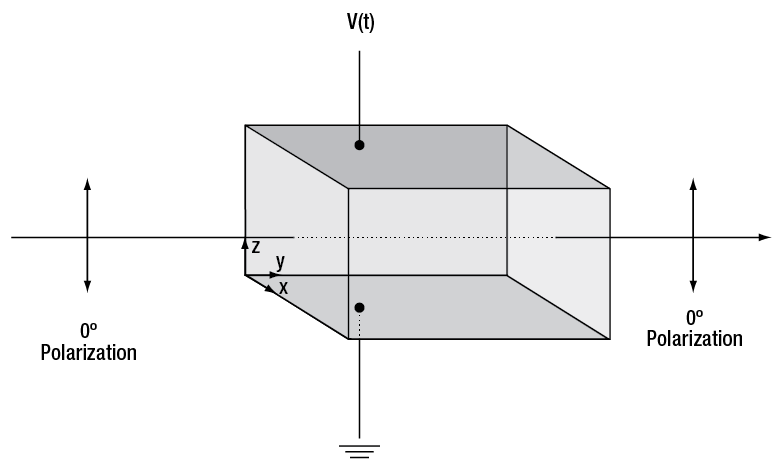
\includegraphics[width=8cm]{src/ElectroOpticKerr.png}
    \caption{Kerr效应装置图}
\end{figure}

某些各向同性的物质, 在外电场作用下, 具有双折射特性, 谓Kerr效应. 感生折射率与$E^2$成正比, $\+vE$的方向为光轴.
\begin{align*}
    \Delta n &= n_o - n_e = BE^2, \quad \Delta\varphi = \frac{2\pi}{\lambda}\Delta n\cdot d = 2\pi BE^2 \frac{d}{\lambda}.
\end{align*}
若前后摆放两个相互垂直的偏振片, 则
\[ I = \frac{I_0}{2}\pare{1-\cos\Delta\varphi} = I_0 \sin^2 \frac{\Delta\varphi}{2}. \]

\begin{figure}[ht]
    \centering
    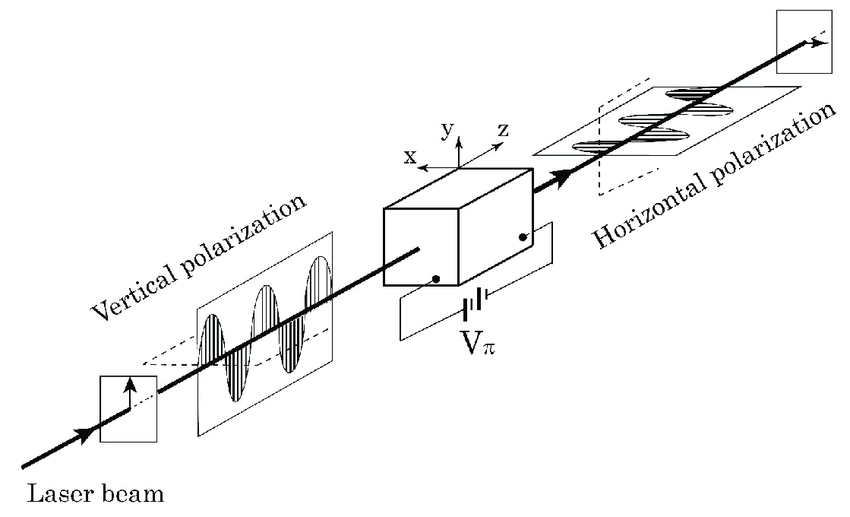
\includegraphics[width=12cm]{src/ElectroOpticPockels.png}
    \caption{Pockels效应装置图}
\end{figure}

一些单轴晶体在外电场中, 光沿着晶体光轴传播, 也能发生双折射, 谓Pockels效应(一阶电光效应).
\begin{align*}
    \Delta n &= n_x - n_y = n_0^3\gamma E, \\
    \Delta \varphi_c &= \frac{2\pi}{\lambda}\pare{n_x - n_y}l = \frac{2\pi}{\lambda}n_0^3 \gamma El = \frac{2\pi}{\lambda}n_o^3 \gamma V.
\end{align*}
若前后摆放两个相互垂直的偏振片, 则
\[ I = \frac{I_0}{2}\pare{1-\cos\Delta\varphi} = I_0 \sin^2 \pare{\frac{\pi}{\lambda}n_o^3 \gamma V}. \]
由此可以用用电压控制光强, 当$V=V_{\lambda/2}$时, 光完全通过, 且$V=V_{\lambda/4}\sim V_{\lambda/2}$附近接近线性.

\begin{remark}
    加横向电场也会有双折射现象(横向Pockels效应), 由于横向宽度小, 可以降低电压.
\end{remark}
\begin{remark}
    通过光纤EOM可以缩短距离以增加电场, 减小所需电压.
\end{remark}
\begin{remark}
    通过并联电路, 串联晶体也可以减小所需电压.
\end{remark}

\paragraph{电光效应的应用} % (fold)
\label{par:电光效应的应用}

可以用于激光光强的调制, 将其变为正弦信号. 
\par
电光晶体EOM对电场的响应时间很短, 可以在$\SI{1e-9}{\second}$内达到半波电压, 以打开或截止光路, 作成高速光开关.
\par
还可以将其用于纯相位调制.

% paragraph 电光效应的应用 (end)

\paragraph{作业} % (fold)
\label{par:作业}

p.214 1, 3, 4, 6 (p.413)

% paragraph 作业 (end)

% subsubsection kerr效应pockels效应 (end)

% subsection 偏振光干涉及其应用 (end)

\subsection{旋光} % (fold)
\label{sub:旋光}

\subsubsection{石英的旋光现象} % (fold)
\label{ssub:石英的旋光现象}

石英晶体中, 线偏光沿着光轴传播, 电矢量振动面旋转; 旋光方向只与晶体有关.
\[ \theta = \alpha l,\quad \alpha = \alpha\pare{\lambda}, \]
其中$\alpha$谓旋光率. 由于$\alpha$是$\lambda$的函数, 故旋光时可能发生旋光色散.
\par
同一种晶体若具有不同的旋光方向则谓之旋光异构体(手性晶体, 对映异构体). 石英有levo(左旋)和dextro(右旋)两种异构体. Pasteur发现酒石酸可能有旋光性, 也可能消旋.

% subsubsection 石英的旋光现象 (end)

\subsubsection{Fresnel对旋光性的解释} % (fold)
\label{ssub:fresnel对旋光性的解释}

线偏光可视为两列反方向旋转的圆偏光合成. 在晶体中, 左旋光和右旋光的折射率不同, 因而在晶体中经过一段距离后一列光比另一列的相位滞后, 从而导致线偏光的振动面旋转.
\par
设左旋光有折射率$n_L$, 右旋光有折射率$n_R$, 则在$t$时刻, 关于$z$点光的相位有
\begin{align*}
    & \varphi_R\pare{t,0} = \varphi_L\pare{t,0} = \varphi_0, \\
    & \varphi_R\pare{t,z} = \varphi_0 - \frac{2\pi}{\lambda}n_R z, \\
    & \varphi_L\pare{t,z} = \varphi_0 - \frac{2\pi}{\lambda}n_L z.
\end{align*}
出晶体后, 左右旋的速度恢复一致, 重新合成为线偏光, 转角为左右旋相位延迟差值的一半,
\[ \varphi = \half\pare{\varphi_R - \varphi_L}. \]
\par
\inlinehardlink{Fresnel复合棱镜}
设$R$晶体满足$n_R<n_L$, $L$晶体满足$n_L < n_R$.
\begin{cenum}
    \item 第一次入射: $R$石英$\rightarrow L$石英.
    \begin{cenum}
        \item 对于$R$光, $R\rightarrow L$, $n$由小变大, $\alpha_R < \alpha_0$.
        \item 对于$L$光, $R\rightarrow L$, $n$由大变小, $\alpha_L > \alpha_0$.
    \end{cenum}
    \item 第二次入射:$L$石英$\rightarrow R$石英.
    \begin{cenum}
        \item 对于$R$光, $n$由大变小, $\alpha_{R}' > \alpha_R$.
        \item 对于$L$光, $n$由小变大, $\alpha_{L}' < \alpha_L$.
    \end{cenum}
\end{cenum}

% subsubsection fresnel对旋光性的解释 (end)

\subsubsection{旋光晶体中的波面} % (fold)
\label{ssub:旋光晶体中的波面}

\inlinehardlink{旋光晶体中的波面}

% subsubsection 旋光晶体中的波面 (end)

\subsubsection{量糖术} % (fold)
\label{ssub:量糖术}

$\theta = \alpha\cdot N\cdot L$.

% subsubsection 量糖术 (end)

\subsubsection{磁致旋光} % (fold)
\label{ssub:磁致旋光}

线偏光通过处于磁场中的介质后, 电矢量的振动面发生旋转,
\[ B = 0,\quad \theta = 0.\quad \theta = VBl. \]
假设光沿着磁场方向传播时发生左旋, 则逆着磁场传播时发生右旋.
\begin{remark}
    这意味着让光通过一个磁致旋光晶体后反射再次经过, 偏振面仍然会有非零的旋转角.
\end{remark}
由磁致旋光可制成单通光闸, 放置反射光损害激光器. \inlinehardlink{S2}
\begin{remark}
    可以由此设计出自动控制溶液浓度的系统.
\end{remark}

\paragraph{作业} % (fold)
\label{par:作业}

p.226 1,2,6 (p.424), 补充题: 采用Faraday旋转镜设计一个两次通过样品的光路(垂直光轴入射, 单轴晶体), 往返光路为同一光路, 且样品要求入射光偏振为特定方向的线偏光.

% paragraph 作业 (end)

% subsubsection 磁致旋光 (end)

% subsection 旋光 (end)

% section 晶体偏振光学 (end)

\end{document}
